%
% BUS 338: Foundations of Innovation - A Course Overview
% Section: User Experience
%
% Author: Jeffrey Leung
%

\section{User Experience}
	\label{sec:user-experience}
\subsection{Research and Insight}
	\label{subsec:user-experience:research-and-insight}
\begin{easylist}
	
& \textbf{User experience research:} Understanding the buyers/users and their needs and goals which can be supported by a solution
	&& Involves discarding initial assumptions
	&& \textbf{Problem research:} Understanding the identity of the buyers/users, their problems, and the context
	&& \textbf{Solution research:} Understanding the usability, feature set, and selling ability of a solution, and the customer satisfaction created

& \textbf{User insight:} Ability to understand the experience of users
	&& Can lead to an opportunity for new products, changes in communication/marketing, etc.
	&& Sources of insight:
		&&& Process of an experience
		&&& Division of labour
		&&& Unique combinations or usages of solutions
		&&& Benefits derived
		&&& Mistakes made
		&&& Frustrations
		&&& Ideal wishes perceived as unachievable
	
& \textbf{Ladder of inference:} Process by which user experience is understood more deeply and in context
\begin{enumerate}
	\item \textit{Observations and experiences} are perceived
	\item \textit{Filters} are applied to select pereceptions
	\item \textit{Meanings} are applied to add cultural and personal context
	\item \textit{Assumptions} are created based on meanings
	\item \textit{Conclusions} are drawn from assumptions
	\item \textit{Beliefs} are created about the subject and affect our future filters and meanings
	\item \textit{Actions} are taken based on beliefs and create new situations which are observed and experienced
\end{enumerate}

& Problems and solutions can be clustered in categories such as feelings, preferences, senses, places, communication, etc.

\end{easylist}
\subsection{Personas}
	\label{subsec:user-experience:personas}
\begin{easylist}

& \textbf{User persona:} Detailed overview of an ideal individual within a market segment, and their personality, preferences, and needs
	&& Criteria:
		&&& Basic demographics: Name, picture, age, gender
		&&& Background: Salary, household income, location, education, family
		&&& Job information: Company, company details (e.g. size, characteristics, main products), role in the company
		&&& Goals and challenges: Difficulties, ideals, current solutions
		&&& Values: Important factors, main objections, fears
	&& One persona for each type of buyer (user/technical/economic) and for anyone who is a part of the decision-making process (e.g. champions, influencers, veto powers)

\end{easylist}
\pagebreak
\subsection{Example Persona}
	\label{subsec:user-experience:example-persona}
\begin{easylist}

\begin{LARGE}
	\centerline{\textbf{Jim Davis}}
\end{LARGE}

\begin{figure}[!ht]
	\centering
	\label{fig:jim-davis}
	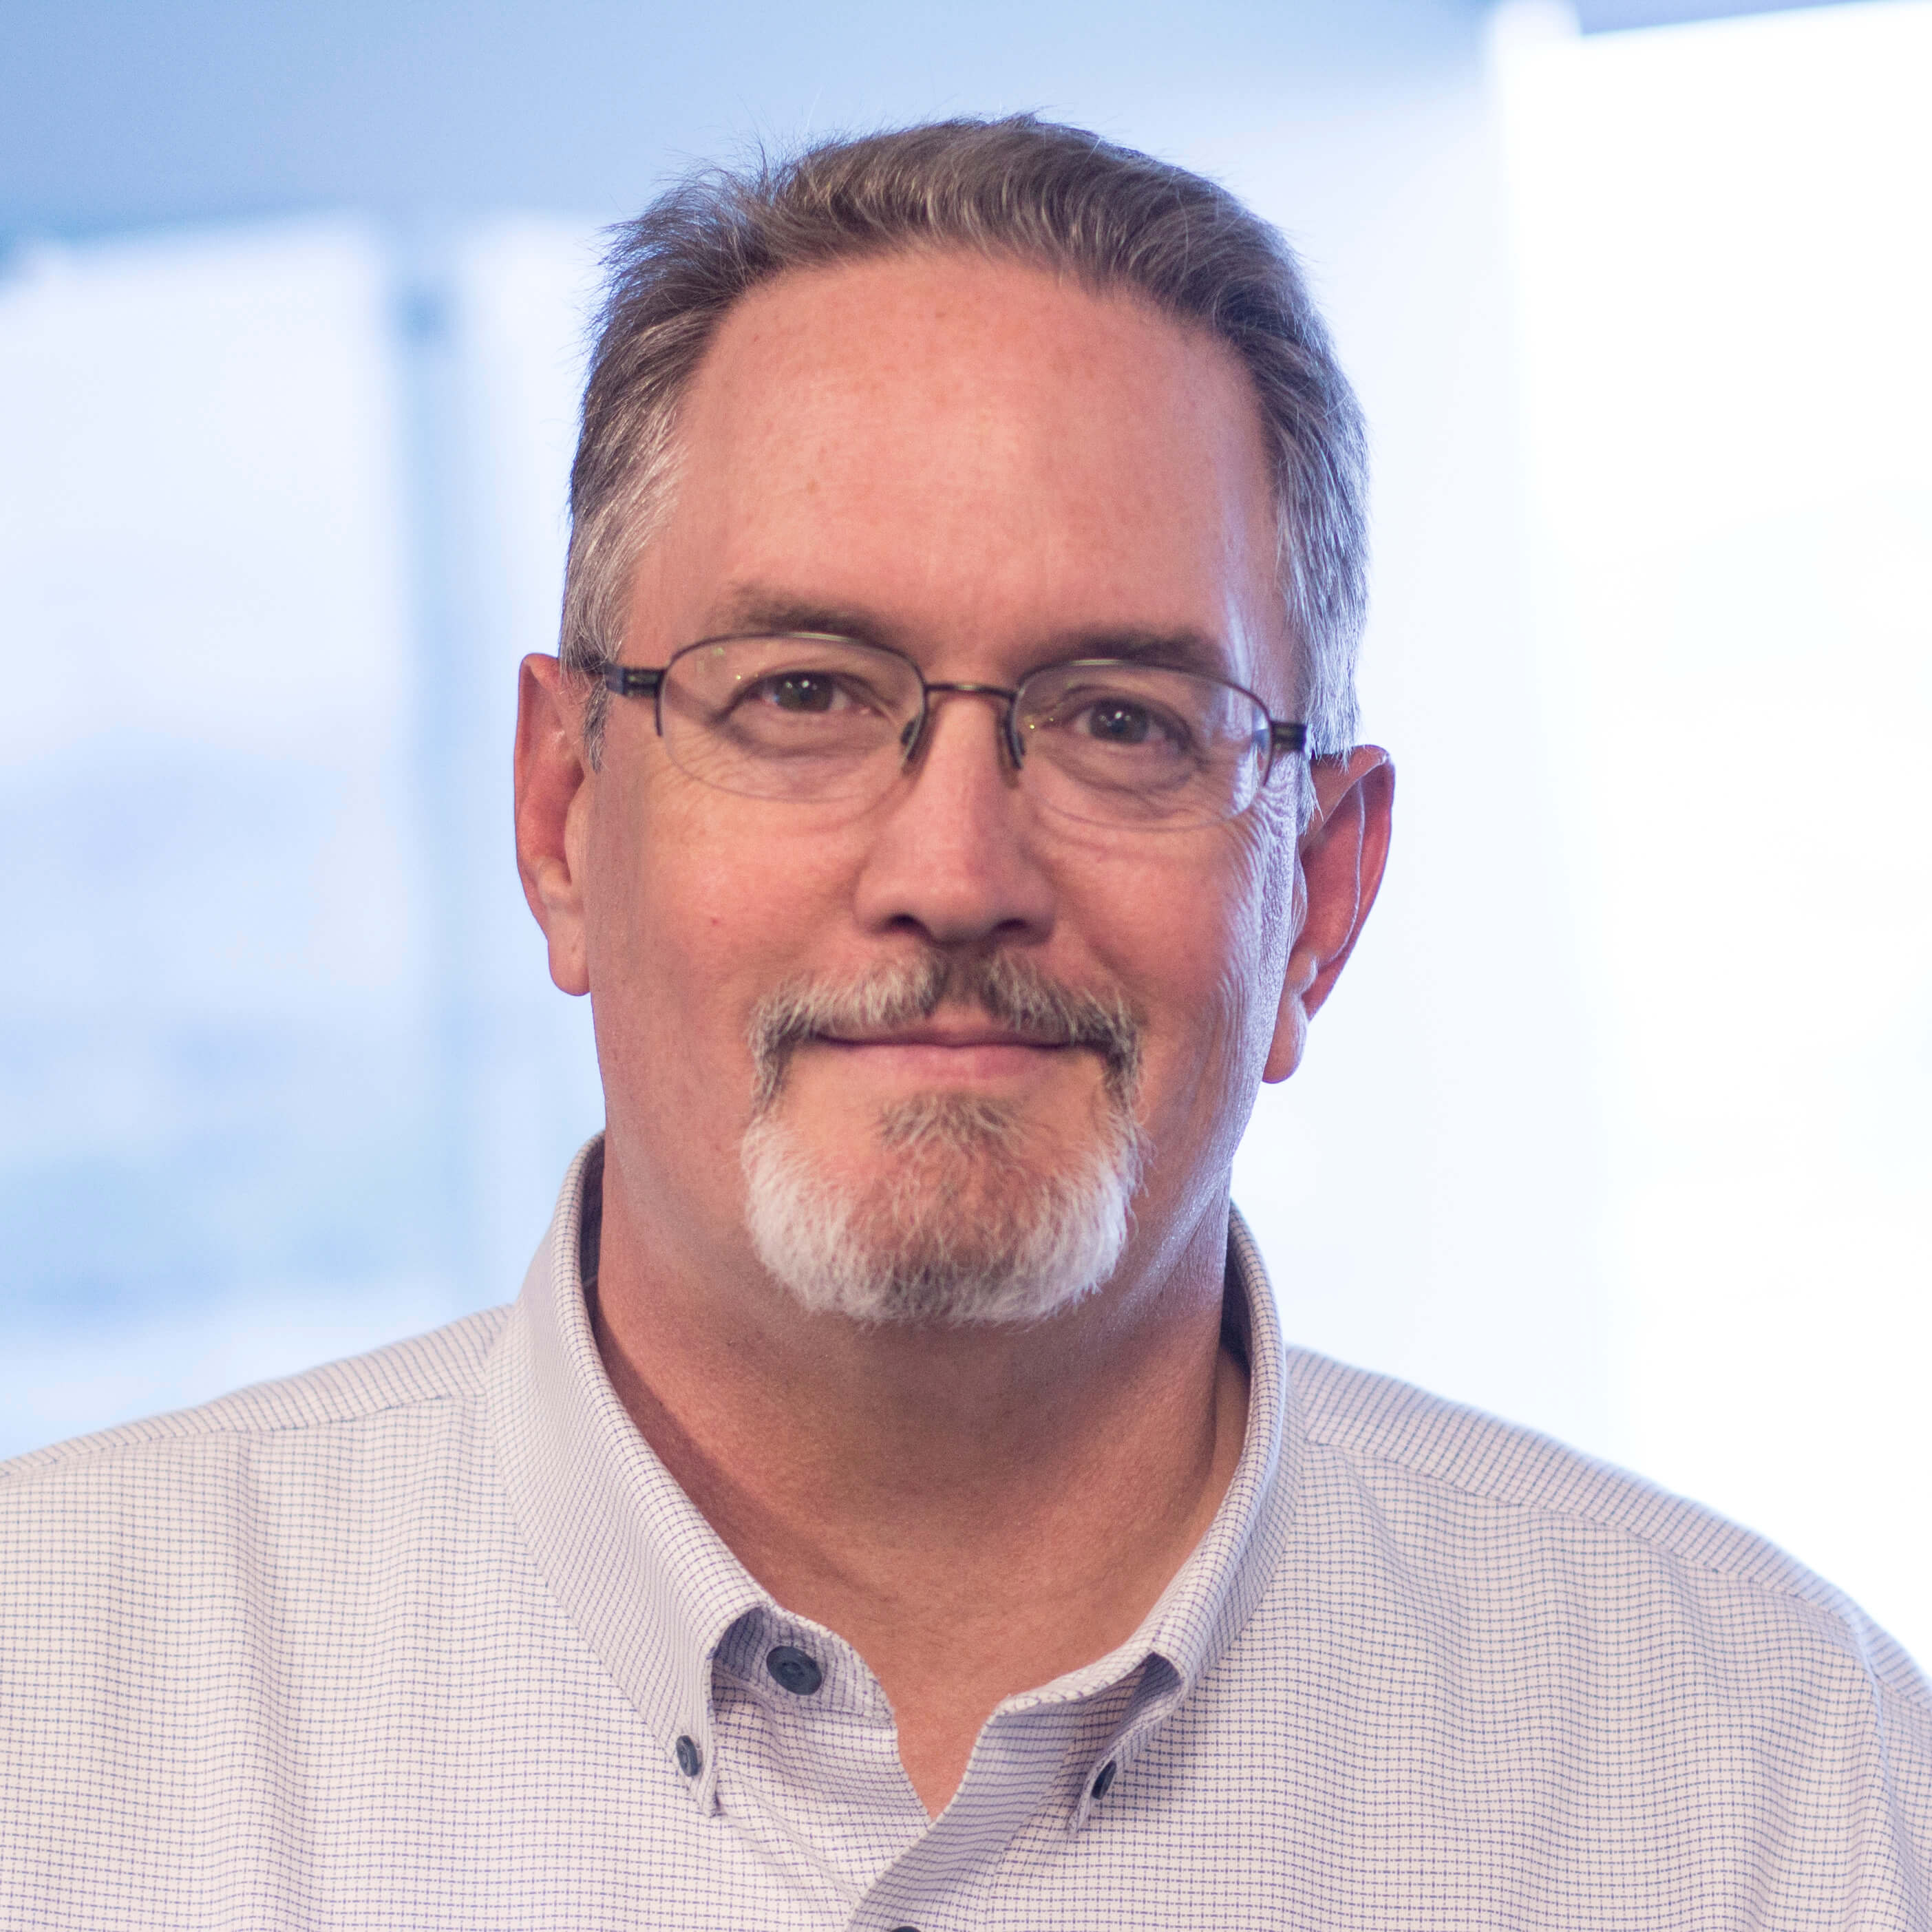
\includegraphics[width=0.4\textwidth]{jim-davis}
\end{figure}

\noindent
\textbf{Biography:} \\
48 years old \\
Married with children (high-school age) \\
Works at Siemens as a Project Manager
Ph.D in Computer Science from MIT \\
Has been managing teams for 15 years. Hands-on. Writes code frequently. \\
Drives a Toyota Prius \\
Carries a Samsung Note

\vspace{1em}

\noindent
\textbf{Behaviours:} \\
Reports to the General Manager \\
Manages the software organization and the associated budget \\
Makes all key decisions on tools and systems for the software organization

\vspace{1em}

\noindent
\textbf{Needs and Goals:} \\
Wants his team to create high-quality code \\
Willing to pay a premium price for the best tools to support his workers

\end{easylist}
\clearpage
